\documentclass[conference]{IEEEtran}
\usepackage{cite}
\usepackage{amsmath,amssymb,amsfonts}
\usepackage{algorithmic}
\usepackage{graphicx}
\usepackage{textcomp}
\usepackage{xcolor}
\usepackage{booktabs}
\usepackage{multirow}
\usepackage{hyperref}
\usepackage{float}
\usepackage{subcaption}
\usepackage{algorithm}
\usepackage{placeins}
\definecolor{pendingcolor}{RGB}{200, 100, 50}
\newcommand{\pending}[1]{\textcolor{pendingcolor}{\textit{[#1]}}}

\begin{document}

\title{How Low Can the Rank Go?}

\author{
\IEEEauthorblockN{Prit Kudale\IEEEauthorrefmark{1}, Naman Dwivedi\IEEEauthorrefmark{2}, Raj Dandekar\IEEEauthorrefmark{2}, Rajat Dandekar\IEEEauthorrefmark{2}, Sreedath Panat\IEEEauthorrefmark{2}}
\IEEEauthorblockA{\IEEEauthorrefmark{1}prit.kudale@gmail.com \quad \IEEEauthorrefmark{2}Vizuara AI Labs, hello@vizuara.com}
}

\maketitle

\begin{abstract}
Low-Rank Adaptation (LoRA) is the default method for parameter-efficient fine-tuning, and its rank $r$ is the single knob that trades adaptation capacity against the number of trainable parameters. Yet how \emph{low} $r$ can be pushed before adaptation degrades has never been characterized with statistical rigor for small encoder classifiers. Prior work either reports isolated point estimates or studies billion-parameter generative models at moderate-to-high ranks without significance testing. We close this gap with a controlled study on DistilBERT-base over two tasks of differing difficulty, SST-2 and AG News, sweeping $r \in \{1,2,4,8,16,32,64\}$ with three seeds per cell, bracketed by a frozen-encoder rank-0 probe and full fine-tuning. We define the \emph{minimum viable rank} as the smallest $r$ whose accuracy is statistically indistinguishable (Welch $t$-test, $\alpha{=}0.05$) from both full fine-tuning and high-rank LoRA. The rank floor is strikingly low and tracks task difficulty: $r{=}4$ on SST-2 (0.11\% of parameters) and $r{=}32$ on AG News under strict equivalence ($r{\approx}4$ under a 0.5\% practical tolerance). Even $r{=}1$, with only 18{,}432 adapter parameters (0.027\% of the model), recovers 59 to 72\% of the probe-to-full-fine-tuning gap. The only regime in which adaptation truly fails is rank 0. The floor is robust to the LoRA scaling rule and, remarkably, to data scarcity: at 500 to 10{,}000 training examples, low-rank LoRA matches or exceeds full fine-tuning. We release all code and the full 162-run result ledger.
\end{abstract}

\begin{IEEEkeywords}
parameter-efficient fine-tuning, LoRA, low-rank adaptation, transformers, text classification, model compression
\end{IEEEkeywords}

\section{Introduction}
Adapting large pretrained transformers to downstream tasks by full fine-tuning is storage and serving expensive, because every task requires a separate copy of all model weights. Parameter-efficient fine-tuning (PEFT) addresses this by updating only a small set of parameters. Low-Rank Adaptation (LoRA)~\cite{hu2021lora} has become the dominant PEFT method: it freezes the pretrained weight $W_0$ and learns a low-rank update $\Delta W = BA$ scaled by $\alpha/r$, where the rank $r$ is far smaller than the matrix dimensions. The theoretical motivation predates LoRA. Work on the intrinsic dimension of objective landscapes~\cite{li2018intrinsic} and of language-model fine-tuning~\cite{aghajanyan2020intrinsic} showed that pretrained models can be adapted within a surprisingly small subspace, with as few as roughly 200 parameters reaching 90\% of full fine-tuning quality on MRPC.

Despite this, the precise lower boundary of the rank has not been mapped. The original LoRA paper reports the striking observation that ``a rank as small as one suffices'' for adapting the query and value projections, but only as point estimates on large models, without multiple seeds, significance testing, a rank-0 reference, or a module-placement study. Subsequent work has largely pushed in the opposite direction: AdaLoRA~\cite{zhang2023adalora}, DoRA~\cite{liu2024dora}, VeRA~\cite{kopiczko2023vera}, and rsLoRA~\cite{kalajdzievski2023rslora} refine how a rank budget is parameterized, allocated, or scaled, while recent rank trade-off studies~\cite{biderman2024lora,rathore2025rank} examine billion-parameter generative decoders at rank $r \geq 8$ and explicitly report no confidence intervals or significance tests. As a result, there is no clean, statistically grounded characterization of the rank floor for the small encoder classifiers that dominate practical text-classification deployments.

We provide that characterization. Using DistilBERT-base~\cite{sanh2019distilbert} on SST-2 (easy, binary) and AG News (harder, four-way), we sweep the very-low-rank regime with three seeds per configuration, bracket it with a frozen-encoder probe (the rank-0 analogue) and full fine-tuning, and report accuracy together with the number and percentage of trainable parameters and the training time. A central methodological choice is to separate the fixed cost of the newly initialized classification head from the adapter parameters that the rank actually controls, so the rank floor is measured cleanly (Section~\ref{sec:method}). Figure~\ref{fig:overview} summarizes the setup.

\textbf{Contributions.}
\begin{enumerate}
\item We give the first statistically grounded characterization of the LoRA rank floor for small encoder classifiers, defining a \emph{minimum viable rank} via a Welch $t$-test against both full fine-tuning and high-rank LoRA, with 95\% confidence intervals over three seeds.
\item We establish a difficulty-to-floor relationship: the minimum viable rank is $4$ on SST-2 (0.11\% of parameters) and $32$ on AG News under strict statistical equivalence, or approximately $4$ under a practical 0.5\% tolerance. Even rank 1, with 0.027\% of parameters, closes 59 to 72\% of the probe-to-full-fine-tuning gap.
\item We run two orthogonal ablations, on the $\alpha$-scaling rule and on attention-only versus attention-plus-MLP module placement, showing the floor is scaling robust and that placing rank across more modules trades rank for parameters.
\item We show through a data-efficiency study that the floor stays low under data scarcity, and that low-rank LoRA matches or exceeds full fine-tuning at 500 to 10{,}000 training examples. All code and the 162-run ledger are released.
\end{enumerate}

The remainder of the paper reviews related work (Section~\ref{sec:related}), formalizes the method and the minimum viable rank (Section~\ref{sec:method}), describes the experimental setup (Section~\ref{sec:setup}), presents results and ablations (Section~\ref{sec:results}), and discusses limitations and conclusions (Sections~\ref{sec:limitations} and~\ref{sec:conclusion}).

\begin{figure*}[t]
\centering
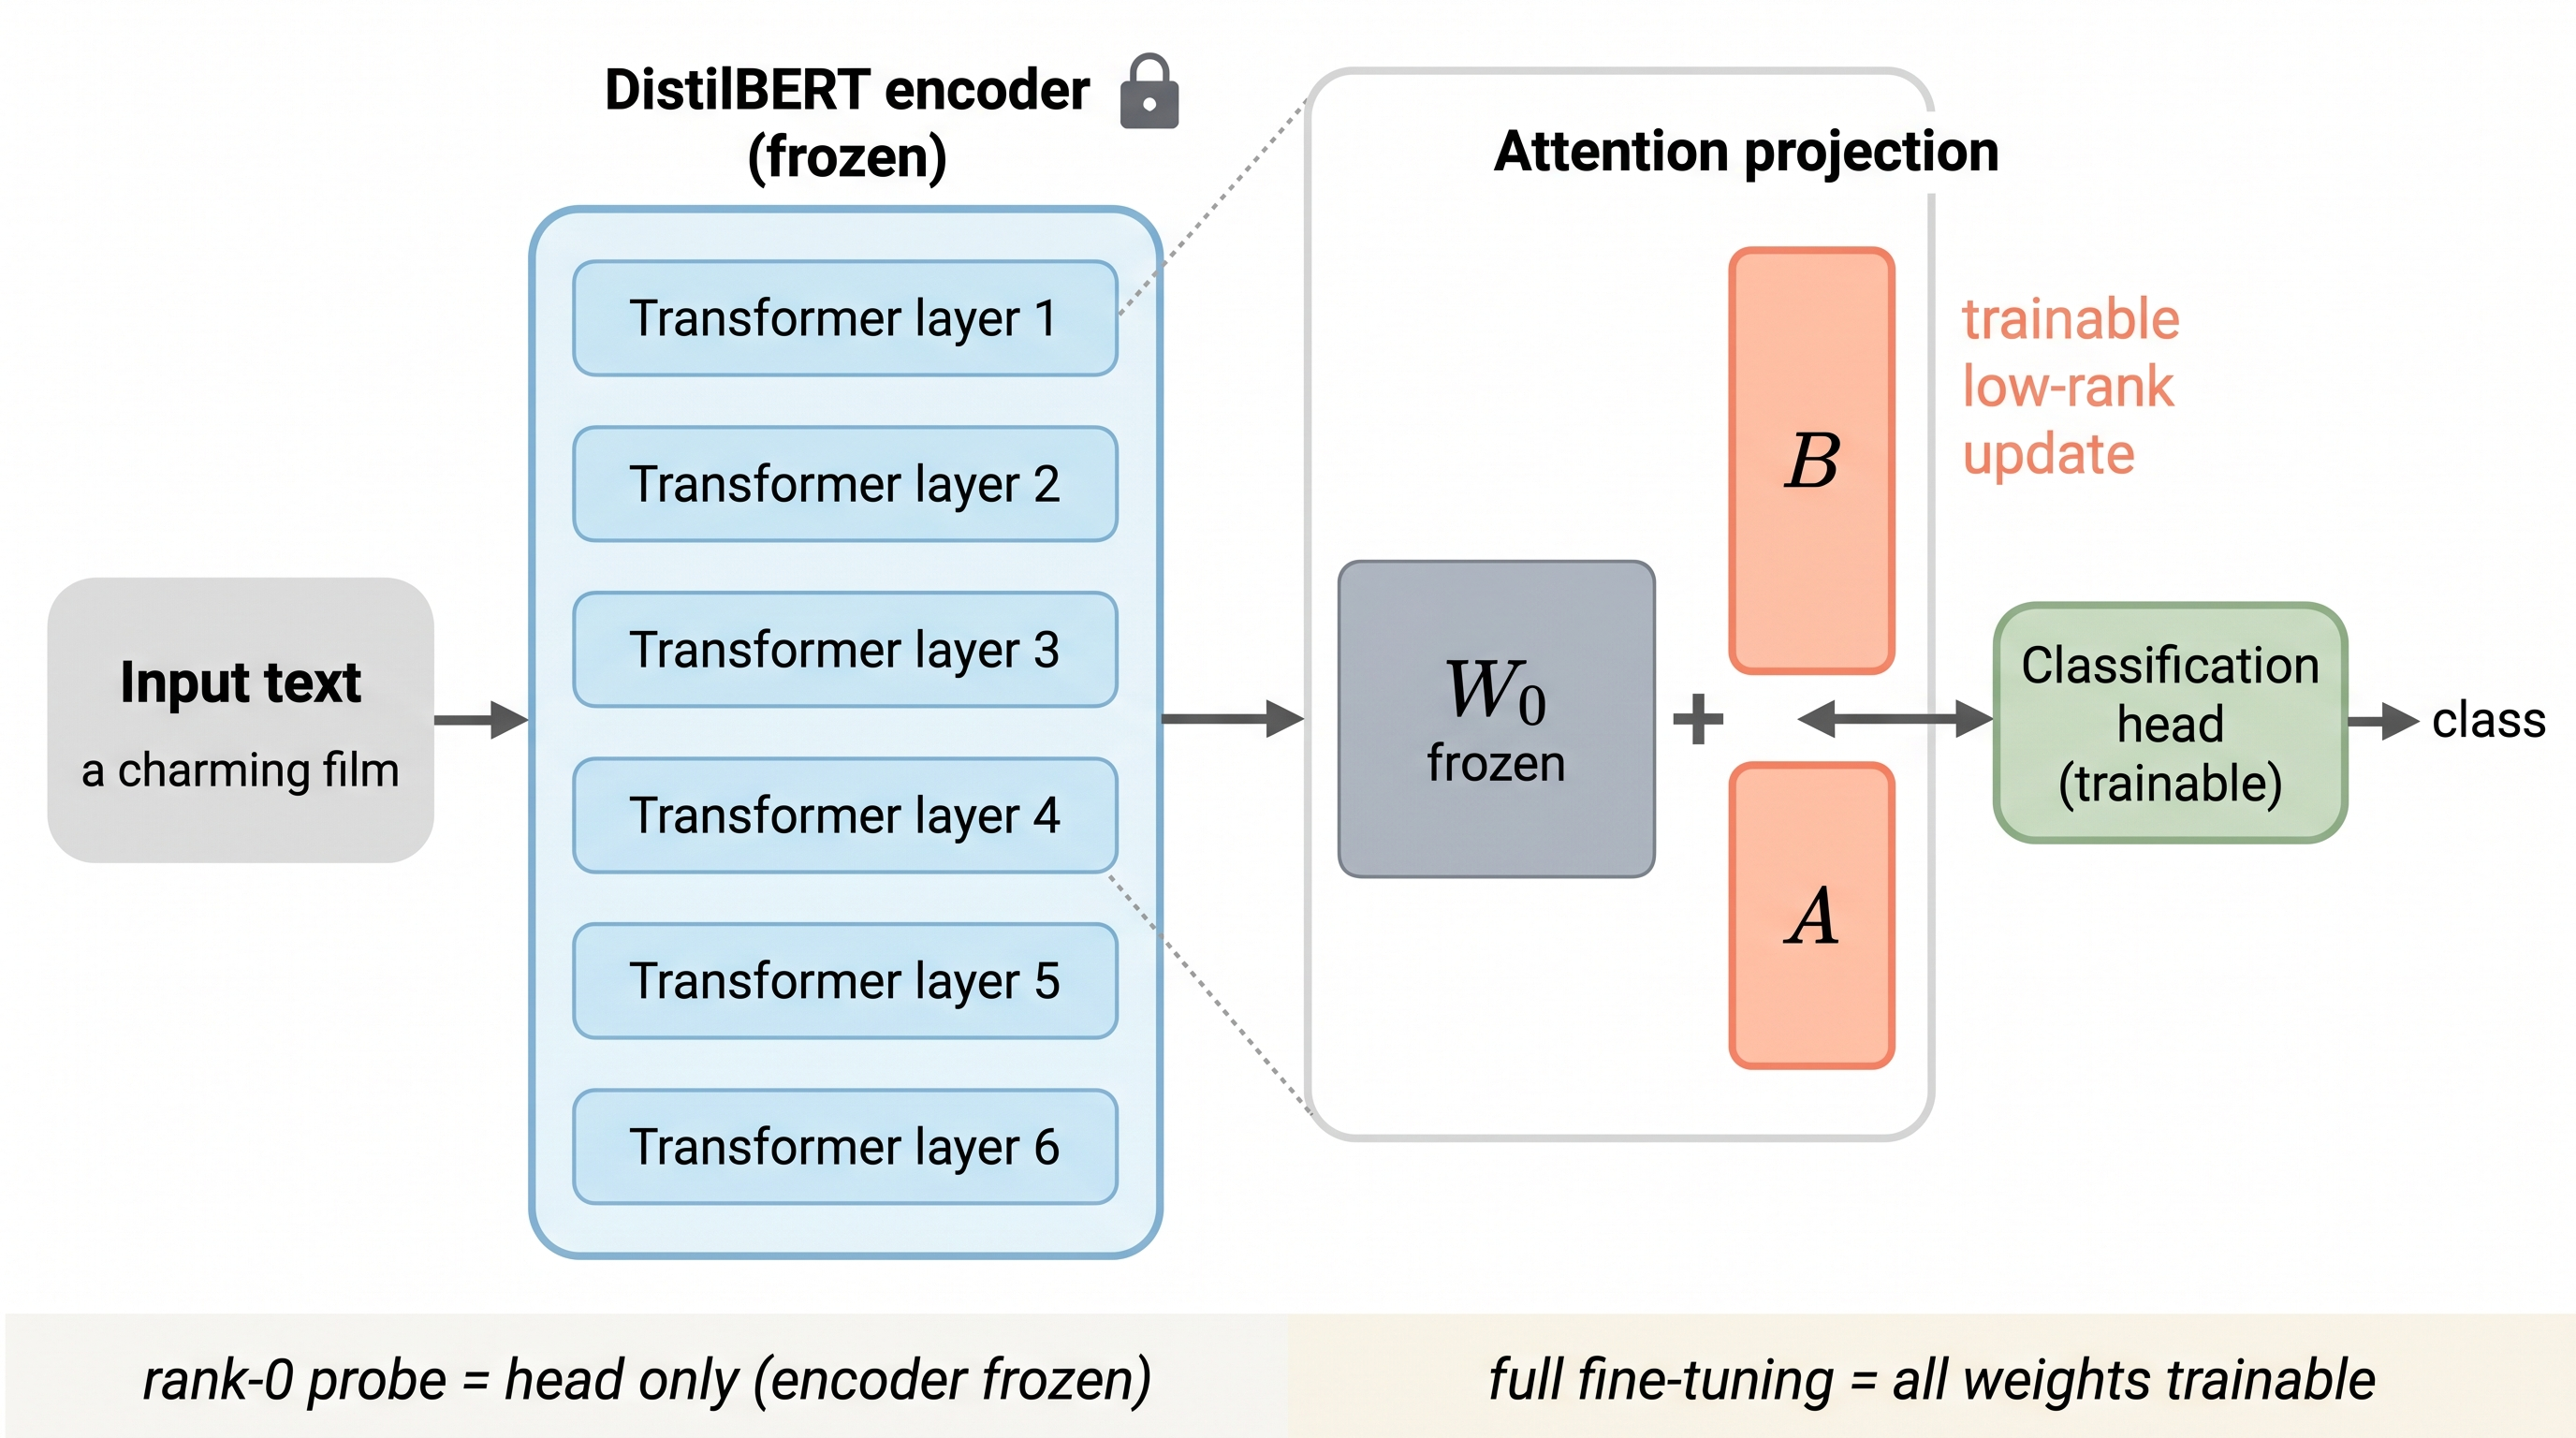
\includegraphics[width=0.88\textwidth]{figures/output/fig2_method_paperbanana.png}
\caption{LoRA adaptation of a small encoder. The pretrained DistilBERT backbone is frozen; a rank-$r$ update $\Delta W = (\alpha/r) BA$ is added to the attention query and value projections. The classification head is a fixed trainable cost present in every configuration. The rank-0 probe (head only) and full fine-tuning (all weights trainable) bracket the rank sweep.}
\label{fig:overview}
\end{figure*}

\section{Background and Related Work}
\label{sec:related}

\subsection{Parameter-Efficient Fine-Tuning}
PEFT methods fall into a few families~\cite{lialin2023scaling,xin2024survey}. Additive methods insert new trainable modules, such as the bottleneck adapters of Houlsby et al.~\cite{houlsby2019adapter}, which reach within 0.4\% of full fine-tuning on GLUE while adding only 3.6\% parameters per task. Selective methods train a subset of existing parameters; the limiting case is a frozen-encoder linear probe that trains only the classification head, which serves as our rank-0 reference. Reparameterization methods, of which LoRA is the canonical instance, learn a structured low-rank update that can be merged into the base weights at inference time with no added latency.

\subsection{LoRA and Its Variants}
LoRA~\cite{hu2021lora} freezes $W_0$ and learns $\Delta W = BA$ with $B \in \mathbb{R}^{d \times r}$ and $A \in \mathbb{R}^{r \times k}$, scaled by $\alpha/r$. Variants modify this recipe along different axes. AdaLoRA~\cite{zhang2023adalora} parameterizes the update in singular-value form and prunes unimportant directions to allocate a fixed budget non-uniformly. DoRA~\cite{liu2024dora} decomposes weights into magnitude and direction and applies LoRA only to the direction. VeRA~\cite{kopiczko2023vera} shares frozen random matrices and learns tiny scaling vectors, reaching 0.043M trainable parameters on GLUE. rsLoRA~\cite{kalajdzievski2023rslora} replaces the $\alpha/r$ scaling with $\alpha/\sqrt{r}$ to stabilize gradients as the rank grows. QLoRA~\cite{dettmers2023qlora} combines 4-bit quantization with LoRA to fit very large models in memory. These methods almost all explore how to spend or scale a rank budget, rather than how small the rank can be.

\subsection{How Low Can the Rank Go?}
The intrinsic-dimension line of work~\cite{li2018intrinsic,aghajanyan2020intrinsic} predicts that the adaptation subspace is small but uses random projections rather than structured LoRA. The LoRA paper hints that rank 1 suffices on some tasks, but without statistical analysis. Biderman et al.~\cite{biderman2024lora} show that on hard generative tasks full fine-tuning finds perturbations of much higher rank than typical LoRA, while LoRA forgets less and acts as a regularizer. Rathore et al.~\cite{rathore2025rank} sweep $r \in \{8,\dots,128\}$ on large instruction-tuned decoders and find no universally best rank, again without significance testing. None of these characterizes the very-low-rank floor for small encoder classifiers with seeds, confidence intervals, a rank-0 bracket, and difficulty stratification, which is the gap we address.

\section{Methodology}
\label{sec:method}

\subsection{Problem Formulation}
For a frozen pretrained weight $W_0 \in \mathbb{R}^{d \times k}$, LoRA learns an additive update
\begin{equation}
W = W_0 + \frac{\alpha}{r} B A, \quad B \in \mathbb{R}^{d \times r}, \ A \in \mathbb{R}^{r \times k},
\end{equation}
with $r \ll \min(d,k)$. The effective scaling factor is $s = \alpha/r$ for standard LoRA and $s = \alpha/\sqrt{r}$ for rsLoRA~\cite{kalajdzievski2023rslora}:
\begin{equation}
s_{\mathrm{std}} = \frac{\alpha}{r}, \qquad s_{\mathrm{rs}} = \frac{\alpha}{\sqrt{r}}.
\end{equation}
Applying LoRA to $m$ attention projection matrices in each of $L$ transformer layers yields an adapter-parameter count
\begin{equation}
P_{\mathrm{adapt}} = L \cdot m \cdot r \cdot (d_{\mathrm{in}} + d_{\mathrm{out}}) = 18{,}432\,r,
\label{eq:params}
\end{equation}
for DistilBERT-base with $L{=}6$, $m{=}2$ (query and value), and $d_{\mathrm{in}}{=}d_{\mathrm{out}}{=}768$.

\subsection{The Fixed-Head Decomposition}
The sequence-classification head of DistilBERT (a pre-classifier $768 \to 768$ followed by a classifier $768 \to C$, totaling approximately 592{,}000 parameters, or 0.88\% of the model) is randomly initialized and must be trainable in every configuration, otherwise the model cannot classify. The head is therefore a constant cost shared by full fine-tuning, LoRA, and the probe alike. We report the adapter parameters of Eq.~\eqref{eq:params} \emph{separately} from the head, because the rank floor concerns adapter capacity on top of a fixed head. The rank-0 probe is exactly the configuration that trains the head only, with the encoder frozen and no adapter.

\subsection{The Minimum Viable Rank}
Let $a(r)$ denote the vector of per-seed accuracies at rank $r$, and let $a_{\mathrm{ref}}$ be a reference (high-rank LoRA at $r{=}64$, or full fine-tuning). We define the minimum viable rank as
\begin{equation}
r^\ast = \min \left\{ r : p_{\mathrm{Welch}}\big(a(r), a_{\mathrm{ref}}\big) > 0.05 \right\},
\label{eq:mvr}
\end{equation}
the smallest rank whose accuracy is not significantly worse than the reference under a two-sided Welch $t$-test, with the additional requirement of overlapping 95\% confidence intervals. We also report a practical variant: the smallest rank within an absolute tolerance $\tau = 0.5\%$ of full fine-tuning.

\subsection{Methods Compared and Training}
We compare full fine-tuning (upper bracket), the frozen-encoder head-only probe (rank-0 lower bracket), and LoRA at $r \in \{1,2,4,8,16,32,64\}$, with $r{=}64$ as the high-rank reference. All models use cross-entropy loss, the AdamW optimizer, a linear schedule with 10\% warmup, mixed-precision training, batch size 32, and maximum sequence length 128. LoRA uses dropout 0.05 and, in the main sweep, attention-only placement on the query and value projections with $\alpha = 2r$ so the effective scaling $s = 2$ is held constant across ranks. Learning rates are $5\times10^{-4}$ for LoRA, $2\times10^{-5}$ for full fine-tuning, and $1\times10^{-3}$ for the probe.

\section{Experimental Setup}
\label{sec:setup}

\subsection{Datasets}
We use two text-classification datasets of differing difficulty, summarized in Table~\ref{tab:datasets}. SST-2 from the GLUE benchmark~\cite{wang2018glue,socher2013sst} is binary sentiment classification; because its test labels are hidden, we report development-set accuracy following standard practice. AG News~\cite{zhang2015agnews} is four-way news-topic classification with a public test split, on which we report test accuracy. Accuracy is the metric for both.

\begin{table}[t]
\caption{Dataset statistics.}
\label{tab:datasets}
\centering
\begin{tabular}{lcccc}
\toprule
Dataset & Task & Classes & Train & Eval \\
\midrule
SST-2 & sentiment & 2 & 67{,}349 & 872 (dev) \\
AG News & topic & 4 & 120{,}000 & 7{,}600 (test) \\
\bottomrule
\end{tabular}
\end{table}

\subsection{Implementation Details}
All experiments run on Modal serverless A100-40GB GPUs using PyTorch 2.4.1, Transformers 4.44.2, PEFT 0.13.2, and Datasets 2.21.0, with \texttt{distilbert-base-uncased} (66.96M parameters) as the backbone. We executed 162 training runs in total (54 core grid, 36 ablation, 72 data-efficiency), each repeated over seeds $\{0,1,2\}$. Per-run metrics, including accuracy, the adapter and total trainable parameter counts, and wall-clock training time, were logged to an append-only ledger that is the single source of truth for every number in this paper.

\subsection{Baselines}
The three baselines are full fine-tuning, which trains all 66.96M parameters and forms the upper bracket; the frozen-encoder probe, which trains only the 0.88\% classification head and forms the rank-0 lower bracket; and standard high-rank LoRA at $r{=}64$, which serves as the reference for the significance test in Eq.~\eqref{eq:mvr}.

\section{Results}
\label{sec:results}

\subsection{The Rank-Floor Curve}
Figure~\ref{fig:floor} is the central result, and Table~\ref{tab:main} gives the full numbers. On SST-2, accuracy rises from the rank-0 probe at 0.8452 to 0.8872 at $r{=}1$ and plateaus near full fine-tuning (0.9029) by $r{=}2$. Rank 4 reaches 0.8979 and is statistically indistinguishable from both full fine-tuning ($p{=}0.41$) and $r{=}64$ ($p{=}0.69$), giving a minimum viable rank of $r^\ast{=}4$. On AG News, accuracy climbs smoothly and monotonically, from the probe at 0.9169 to 0.9446 at $r{=}64$ and 0.9457 for full fine-tuning. Here the seed variance is very small (standard deviation near 0.001), so even the 0.5-point gap at $r{=}8$ is statistically significant; the strict minimum viable rank is $r^\ast{=}32$ ($p{=}0.077$ versus full fine-tuning), while a practical 0.5\% tolerance is met by $r{\approx}4$. Table~\ref{tab:mvr} reports the per-rank significance tests.

\begin{figure*}[t]
\centering
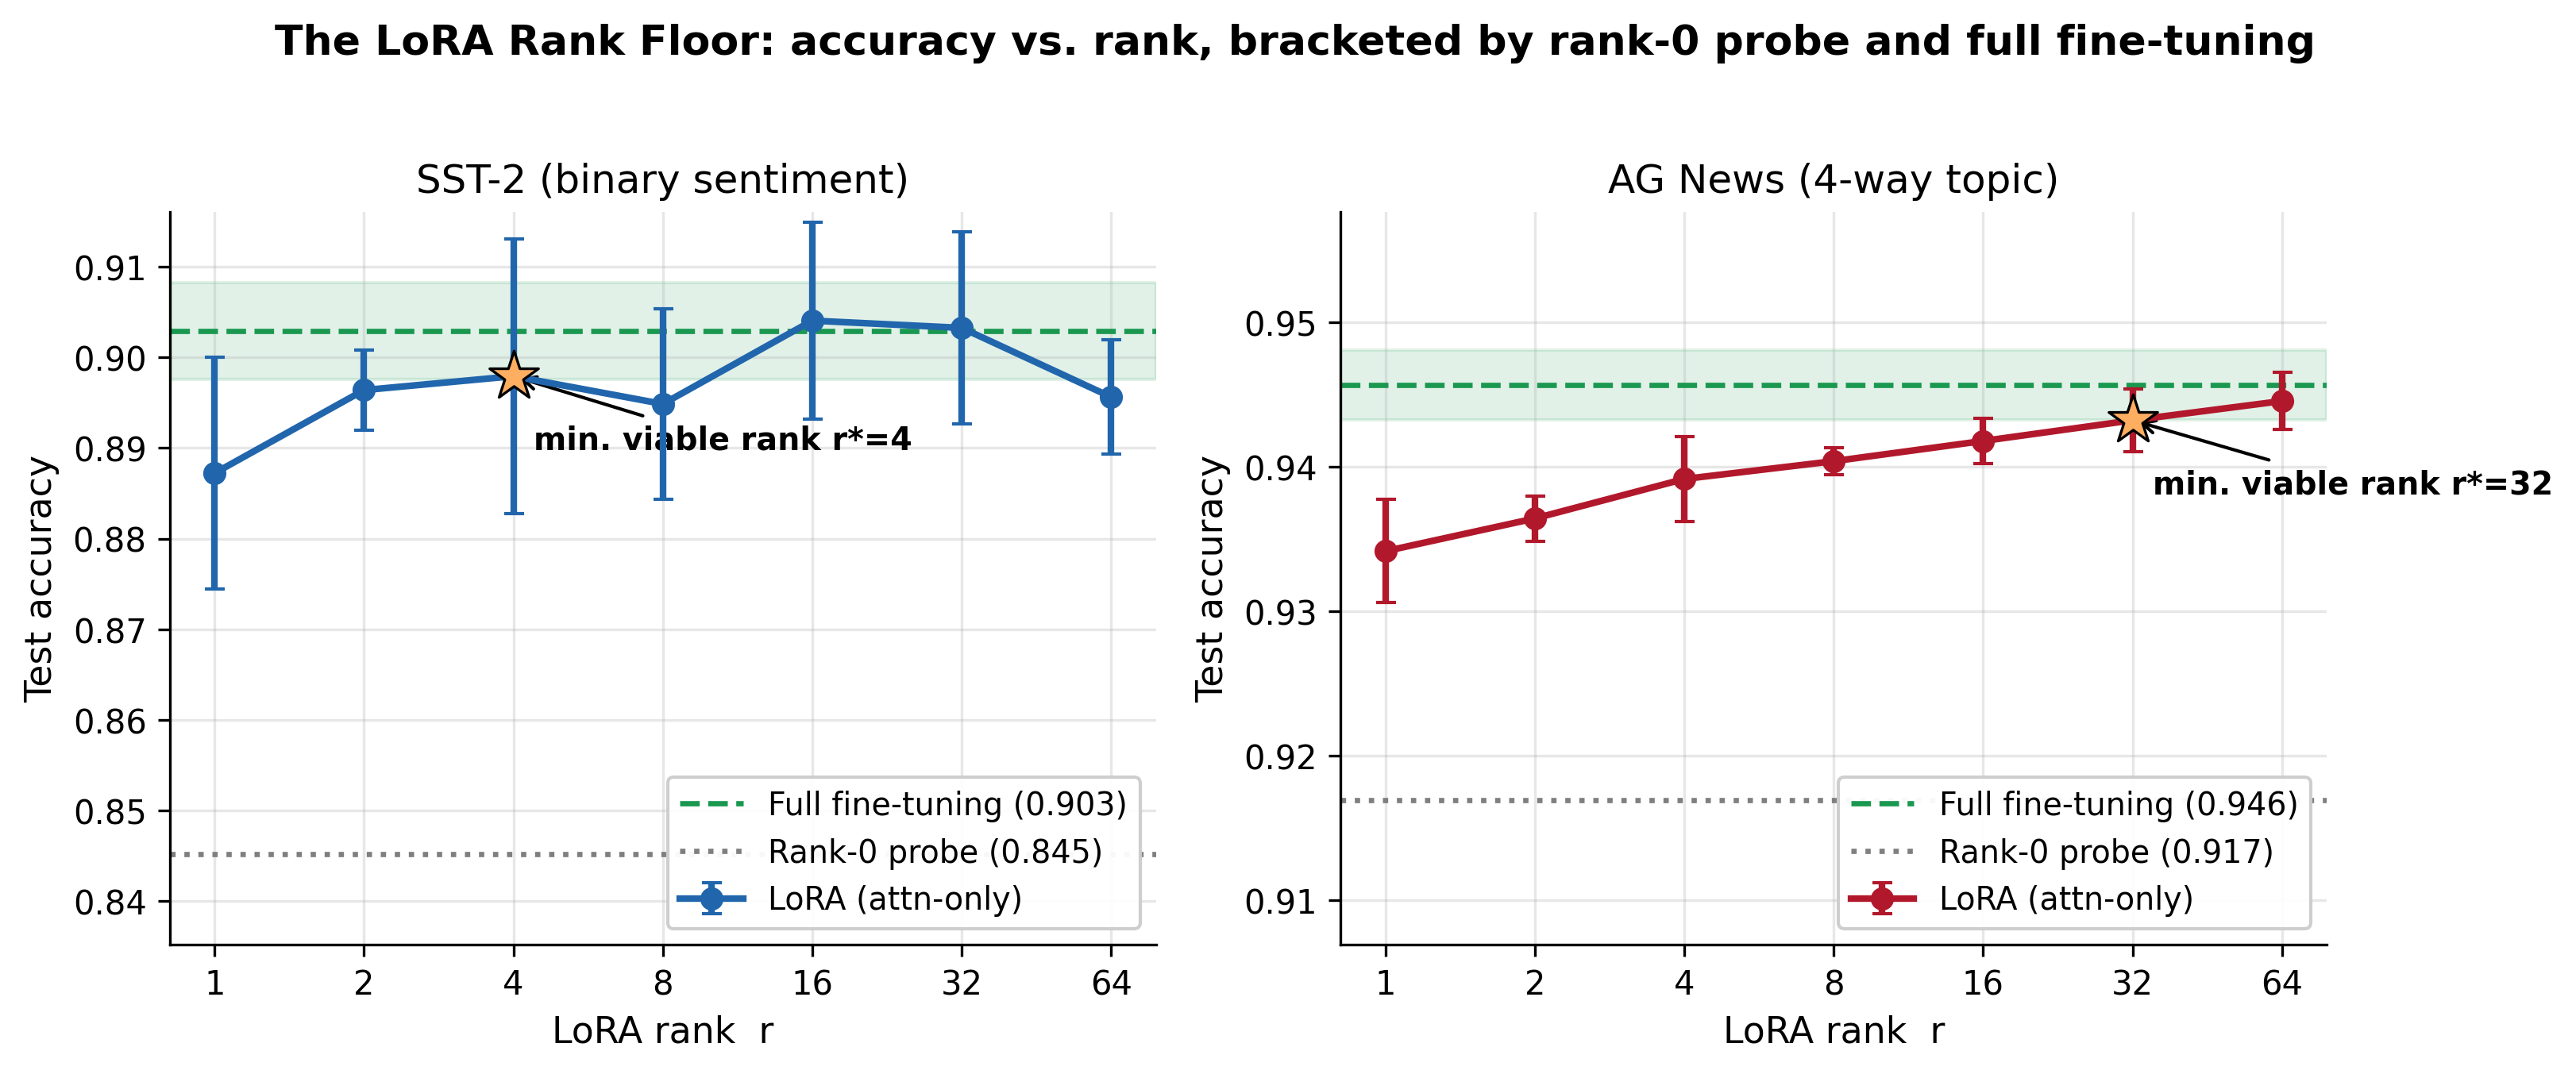
\includegraphics[width=0.97\textwidth]{figures/output/fig1_rank_floor_curve.png}
\caption{The LoRA rank floor. Test accuracy versus rank for DistilBERT-base on SST-2 (left) and AG News (right). Markers are means over three seeds with 95\% confidence intervals; the green band is the full-fine-tuning confidence interval and the dotted line is the rank-0 probe. The star marks the minimum viable rank, the smallest rank statistically indistinguishable from full fine-tuning.}
\label{fig:floor}
\end{figure*}

\begin{table*}[t]
\caption{Main results. Accuracy (mean over three seeds with 95\% confidence interval), adapter parameters from Eq.~\eqref{eq:params}, their percentage of the model, total trainable percentage (adapter plus the fixed head), and mean training time. Best accuracy per dataset in bold.}
\label{tab:main}
\centering
\begin{tabular}{l rrrr r rrrr}
\toprule
& \multicolumn{4}{c}{\textbf{SST-2} (dev accuracy)} & & \multicolumn{4}{c}{\textbf{AG News} (test accuracy)} \\
\cmidrule(lr){2-5} \cmidrule(lr){7-10}
Method & Acc. & Adapter & \% adapt & \% train & & Acc. & Adapter & \% adapt & \% train \\
\midrule
Probe ($r{=}0$) & $0.8452${\scriptsize$\pm.003$} & 0 & 0.000 & 0.884 & & $0.9169${\scriptsize$\pm.002$} & 0 & 0.000 & 0.887 \\
LoRA $r{=}1$ & $0.8872${\scriptsize$\pm.017$} & 18{,}432 & 0.027 & 0.904 & & $0.9342${\scriptsize$\pm.005$} & 18{,}432 & 0.027 & 0.906 \\
LoRA $r{=}2$ & $0.8964${\scriptsize$\pm.006$} & 36{,}864 & 0.055 & 0.931 & & $0.9364${\scriptsize$\pm.002$} & 36{,}864 & 0.055 & 0.933 \\
LoRA $r{=}4$ & $0.8979${\scriptsize$\pm.020$} & 73{,}728 & 0.109 & 0.985 & & $0.9392${\scriptsize$\pm.004$} & 73{,}728 & 0.109 & 0.987 \\
LoRA $r{=}8$ & $0.8949${\scriptsize$\pm.014$} & 147{,}456 & 0.218 & 1.093 & & $0.9404${\scriptsize$\pm.001$} & 147{,}456 & 0.218 & 1.095 \\
LoRA $r{=}16$ & $\mathbf{0.9041}${\scriptsize$\pm.015$} & 294{,}912 & 0.435 & 1.308 & & $0.9418${\scriptsize$\pm.002$} & 294{,}912 & 0.435 & 1.310 \\
LoRA $r{=}32$ & $0.9033${\scriptsize$\pm.014$} & 589{,}824 & 0.866 & 1.735 & & $0.9432${\scriptsize$\pm.003$} & 589{,}824 & 0.866 & 1.737 \\
LoRA $r{=}64$ & $0.8956${\scriptsize$\pm.009$} & 1{,}179{,}648 & 1.716 & 2.578 & & $0.9446${\scriptsize$\pm.003$} & 1{,}179{,}648 & 1.716 & 2.580 \\
Full fine-tuning & $0.9029${\scriptsize$\pm.007$} & --- & --- & 100.0 & & $\mathbf{0.9457}${\scriptsize$\pm.003$} & --- & --- & 100.0 \\
\bottomrule
\end{tabular}
\end{table*}

\begin{table}[t]
\caption{Minimum viable rank. Two-sided Welch $t$-test $p$-values for each rank versus full fine-tuning; indistinguishable when $p>0.05$. The smallest such rank is the minimum viable rank $r^\ast$.}
\label{tab:mvr}
\centering
\begin{tabular}{c cc cc}
\toprule
& \multicolumn{2}{c}{SST-2} & \multicolumn{2}{c}{AG News} \\
\cmidrule(lr){2-3} \cmidrule(lr){4-5}
$r$ & $p$ vs.\ full & indist.? & $p$ vs.\ full & indist.? \\
\midrule
1 & 0.045 & no & 0.002 & no \\
2 & 0.043 & no & 0.001 & no \\
4 & \textbf{0.411} & \textbf{yes} & 0.006 & no \\
8 & 0.120 & yes & 0.012 & no \\
16 & 0.780 & yes & 0.018 & no \\
32 & 0.928 & yes & \textbf{0.077} & \textbf{yes} \\
64 & 0.051 & yes & 0.329 & yes \\
\midrule
\multicolumn{1}{l}{$r^\ast$} & \multicolumn{2}{c}{\textbf{4}} & \multicolumn{2}{c}{\textbf{32} (strict), $\approx$4 (0.5\%)} \\
\bottomrule
\end{tabular}
\end{table}

The efficiency view in Figure~\ref{fig:pareto} reframes these numbers as a Pareto front of accuracy against adapter parameters. Tiny adapters dominate: on both tasks, accuracy rises steeply at the smallest ranks and then flattens, so the marginal value of additional rank collapses almost immediately. Notably, on SST-2 the high-rank $r{=}64$ configuration (0.8956) does not exceed $r{=}16$ (0.9041) or full fine-tuning, indicating that extra rank provides no benefit on the easy task and that the mild non-monotonicity at high rank lies within seed noise.

\begin{figure}[t]
\centering
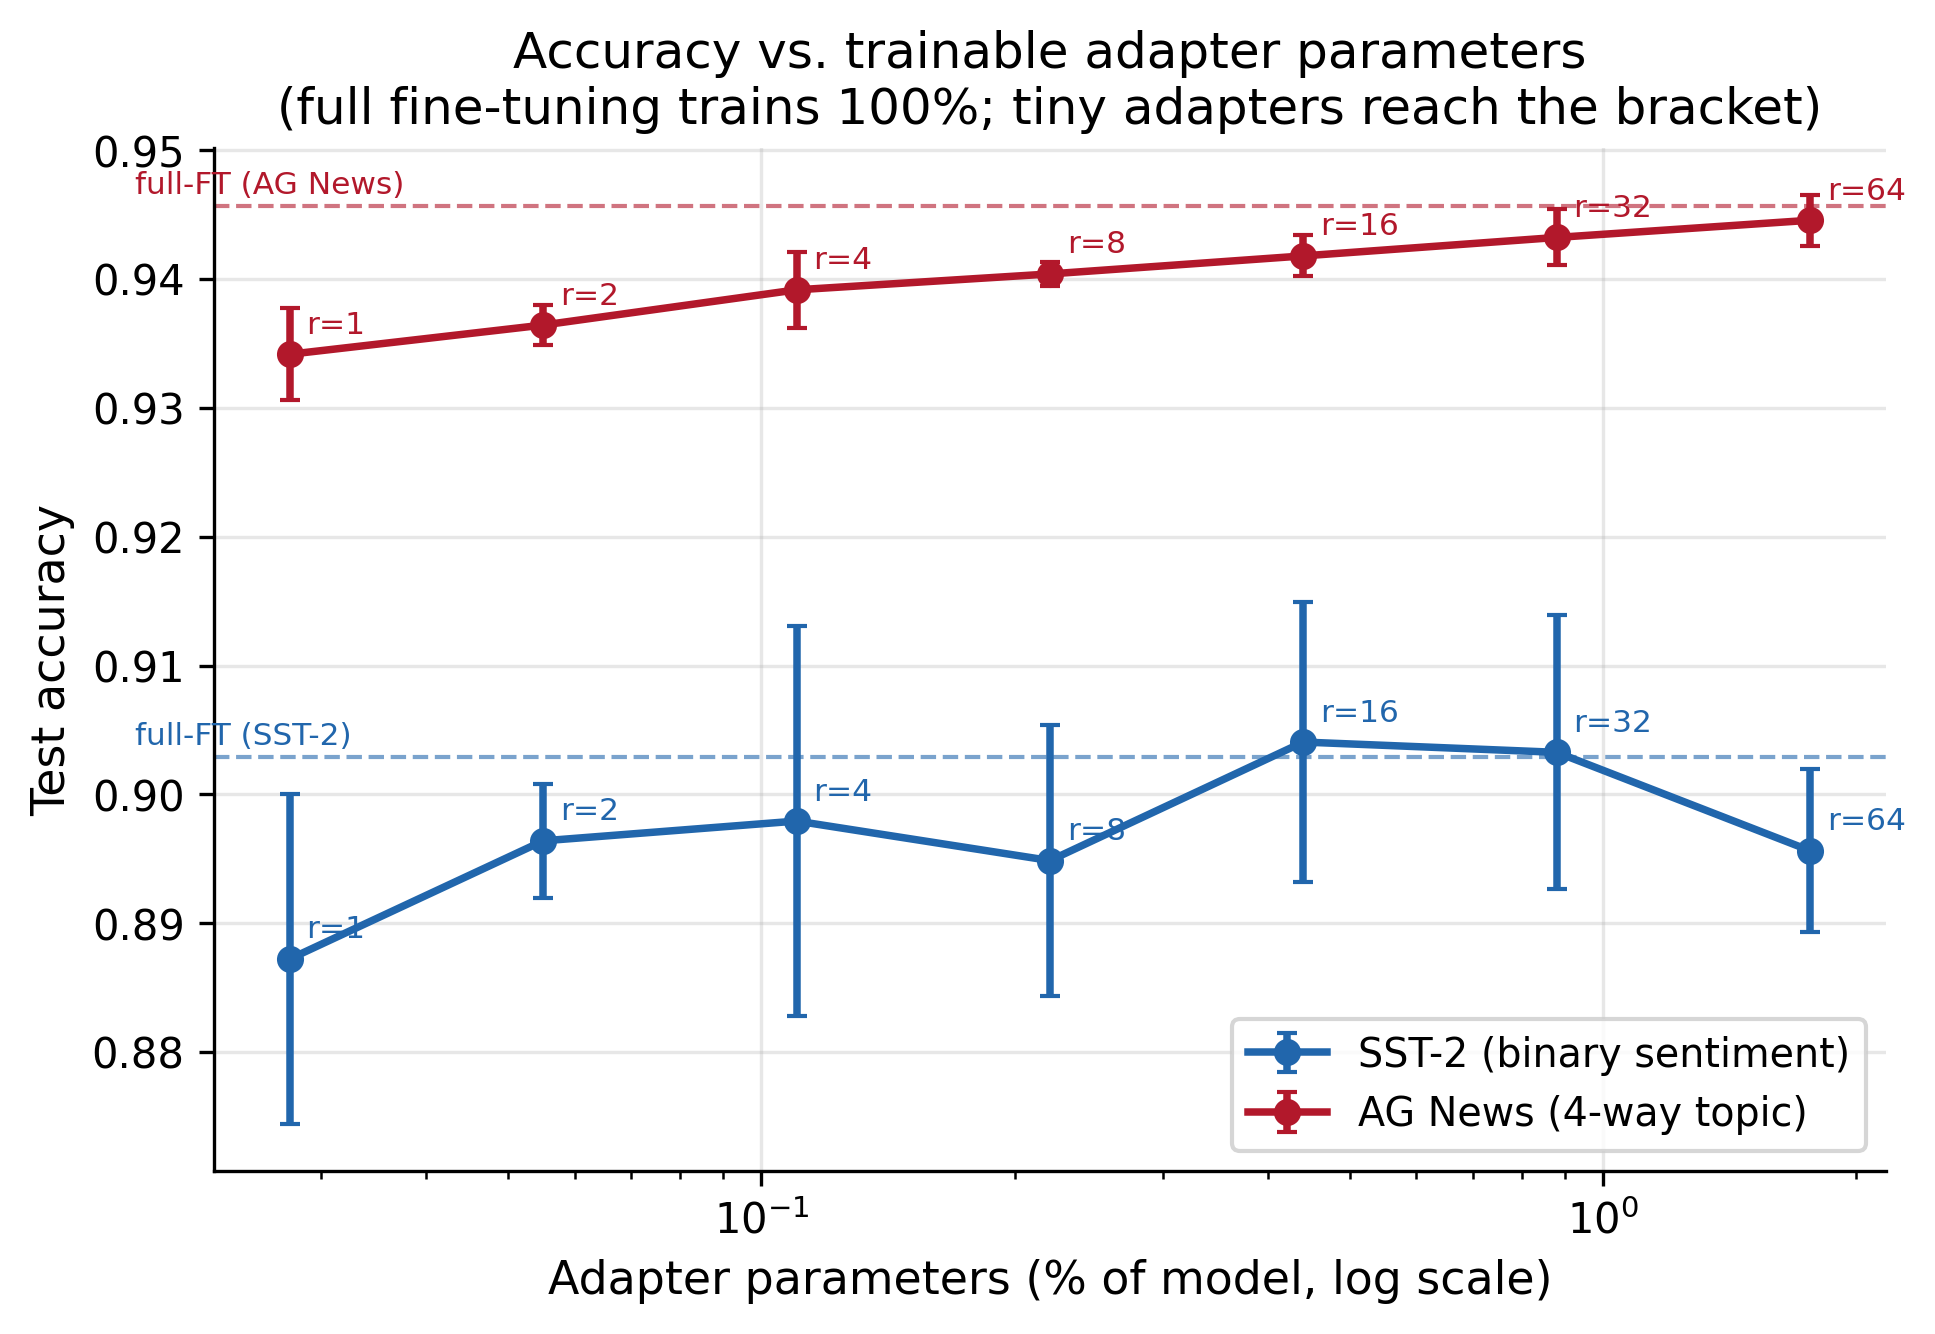
\includegraphics[width=\columnwidth]{figures/output/fig3_accuracy_vs_params.png}
\caption{Accuracy versus adapter parameters as a percentage of the model (log scale). Full fine-tuning trains 100\% of parameters; the dashed lines mark its accuracy. Tiny adapters reach the full-fine-tuning bracket on both tasks.}
\label{fig:pareto}
\end{figure}

\subsection{Ablation: Module Placement}
Figure~\ref{fig:placement} compares attention-only placement against attention-plus-MLP placement (adding the two feed-forward projections) at $r \in \{1,4,16\}$. Placing rank across more modules lowers the floor in rank terms, most visibly at very low rank and on the harder task: AG News attention-plus-MLP at $r{=}16$ reaches 0.9459, matching full fine-tuning (0.9457), whereas attention-only required $r{=}32$. However, attention-plus-MLP costs more adapter parameters per rank ($64{,}512\,r$ versus $18{,}432\,r$), so attention-plus-MLP at $r{=}16$ (1.03M parameters) is larger than attention-only at $r{=}32$ (0.59M). In parameter terms, concentrating low rank on the attention projections remains the most efficient route to the full-fine-tuning bracket. The placement axis therefore trades rank for breadth.

\begin{figure*}[t]
\centering
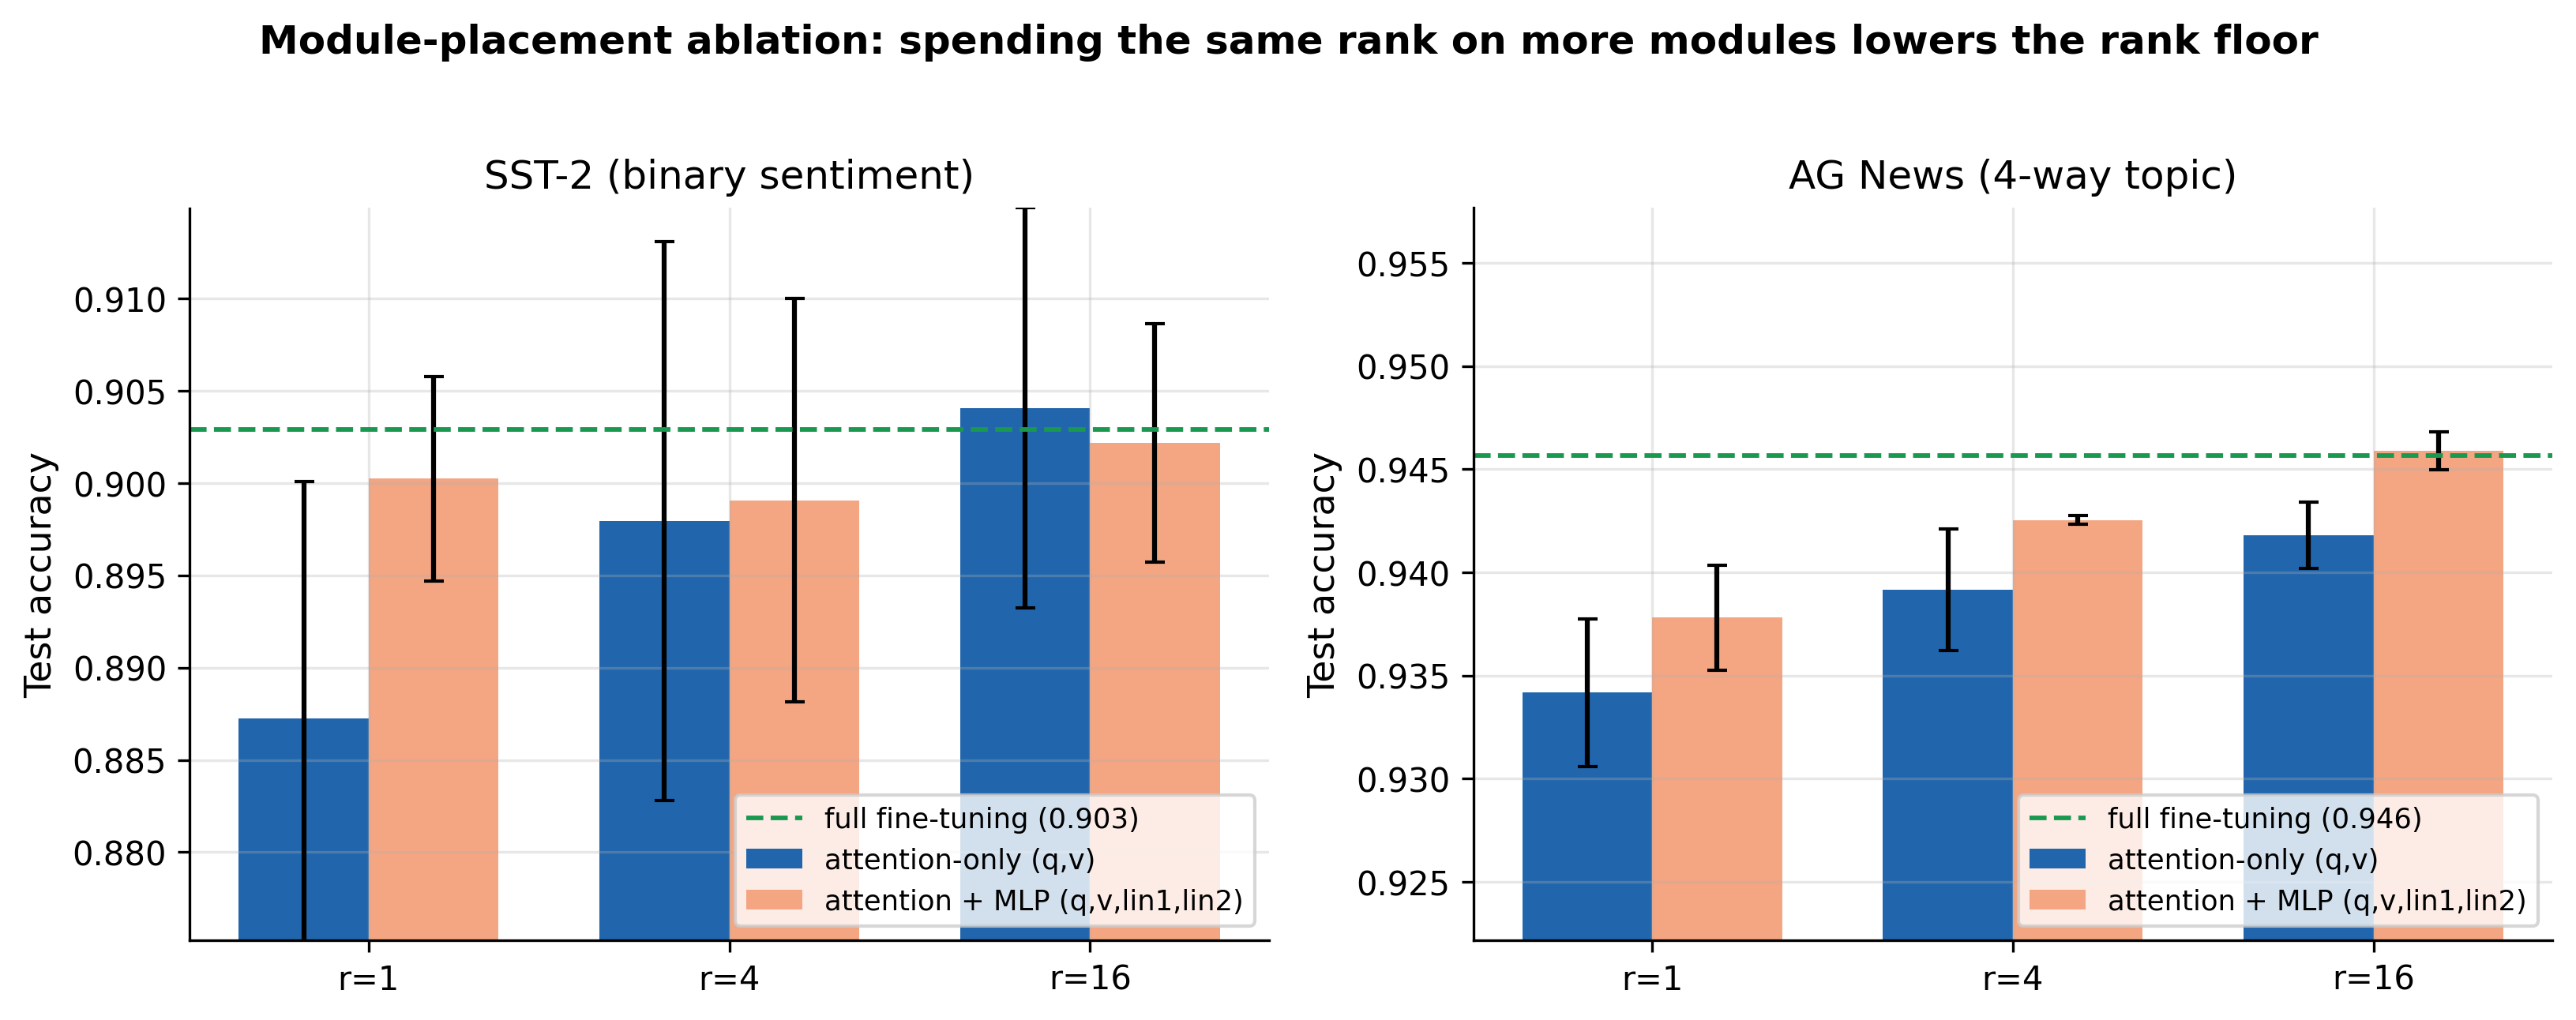
\includegraphics[width=0.95\textwidth]{figures/output/fig4_placement_ablation.png}
\caption{Module-placement ablation. Attention-only versus attention-plus-MLP LoRA at $r \in \{1,4,16\}$, with 95\% confidence intervals and the full-fine-tuning reference. Adding MLP modules lowers the rank floor at a higher parameter cost.}
\label{fig:placement}
\end{figure*}

\subsection{Ablation: Scaling Rule}
Figure~\ref{fig:scaling} compares three scaling rules on SST-2: the constant $s{=}2$ used in the main sweep, a fixed $\alpha{=}8$ (so $s{=}8/r$), and rsLoRA with $\alpha{=}8$ (so $s{=}8/\sqrt{r}$). The floor is largely invariant to the scaling rule. The one exception is at the extreme low rank $r{=}1$, where the larger scaling of the fixed and rsLoRA settings recovers approximately 0.5 points over the constant $s{=}2$ setting (0.8926 versus 0.8872). This indicates that a small part of the rank-1 deficit is an optimization or scaling artifact rather than a pure capacity limit, and that with appropriate scaling even rank 1 nearly closes the gap to full fine-tuning.

\begin{figure}[t]
\centering
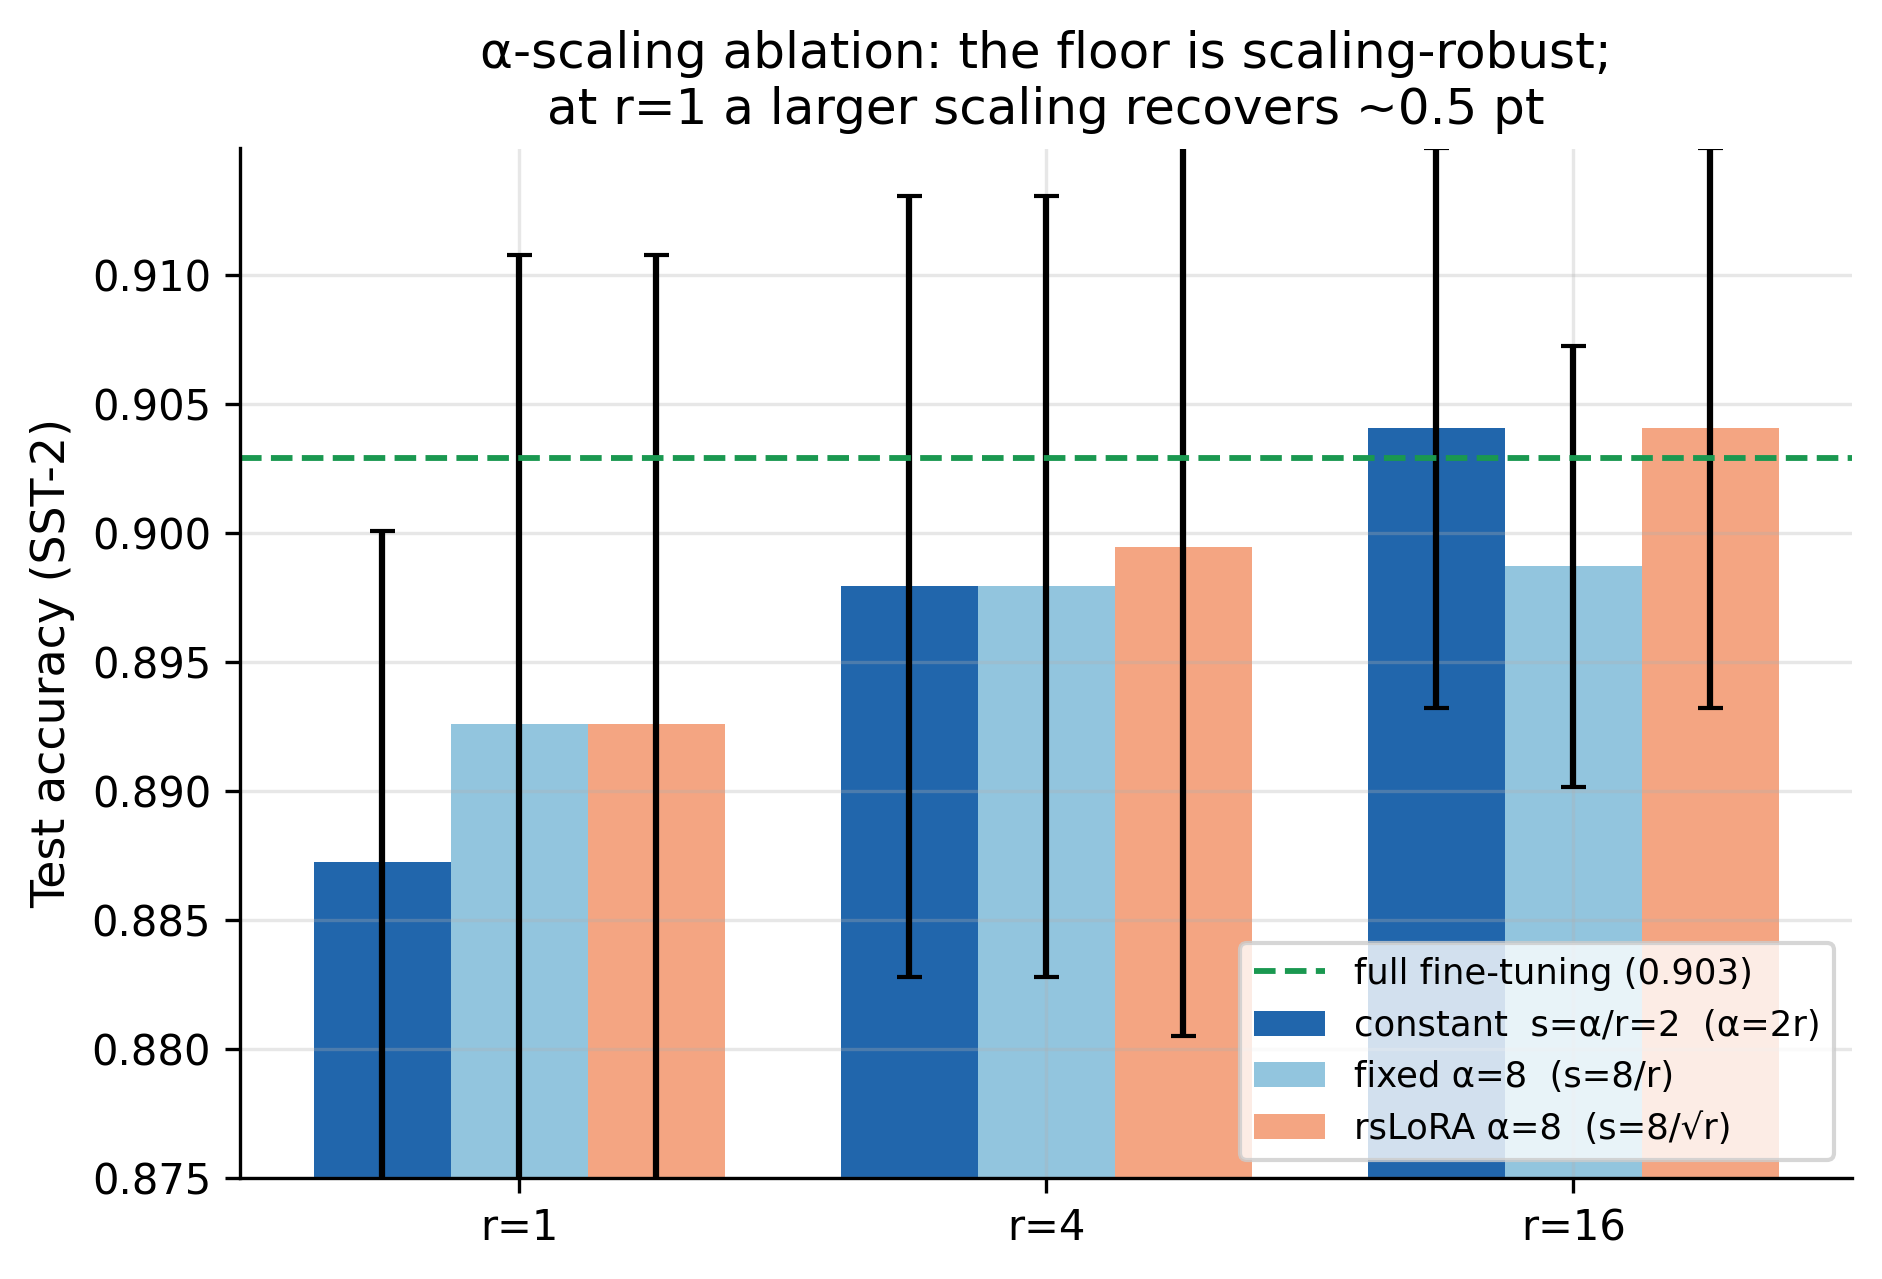
\includegraphics[width=\columnwidth]{figures/output/fig5_scaling_ablation.png}
\caption{$\alpha$-scaling ablation on SST-2. The rank floor is largely robust to the scaling rule; at $r{=}1$, a larger effective scaling recovers roughly 0.5 points.}
\label{fig:scaling}
\end{figure}

\subsection{Data Efficiency}
Figure~\ref{fig:dataeff} asks whether the floor rises when training data is scarce. We subsample the training set to 500, 2{,}000, and 10{,}000 examples and compare full fine-tuning against LoRA at $r \in \{1,4,16\}$. The floor does not rise. On SST-2, the best low-rank LoRA matches or exceeds full fine-tuning at every data size, by 0.8 points at 500 examples, 1.1 points at 2{,}000, and 0.4 points at 10{,}000. On AG News the same trend holds at small data, where attention-plus-MLP-free low-rank LoRA edges full fine-tuning by 0.3 points at 500 examples, converging as data grows. This is consistent with the view that the low-capacity adapter regularizes and overfits less than full fine-tuning when data is limited~\cite{biderman2024lora}. The practical implication is that low rank is not only sufficient but sometimes preferable in the low-data regime.

\begin{figure*}[t]
\centering
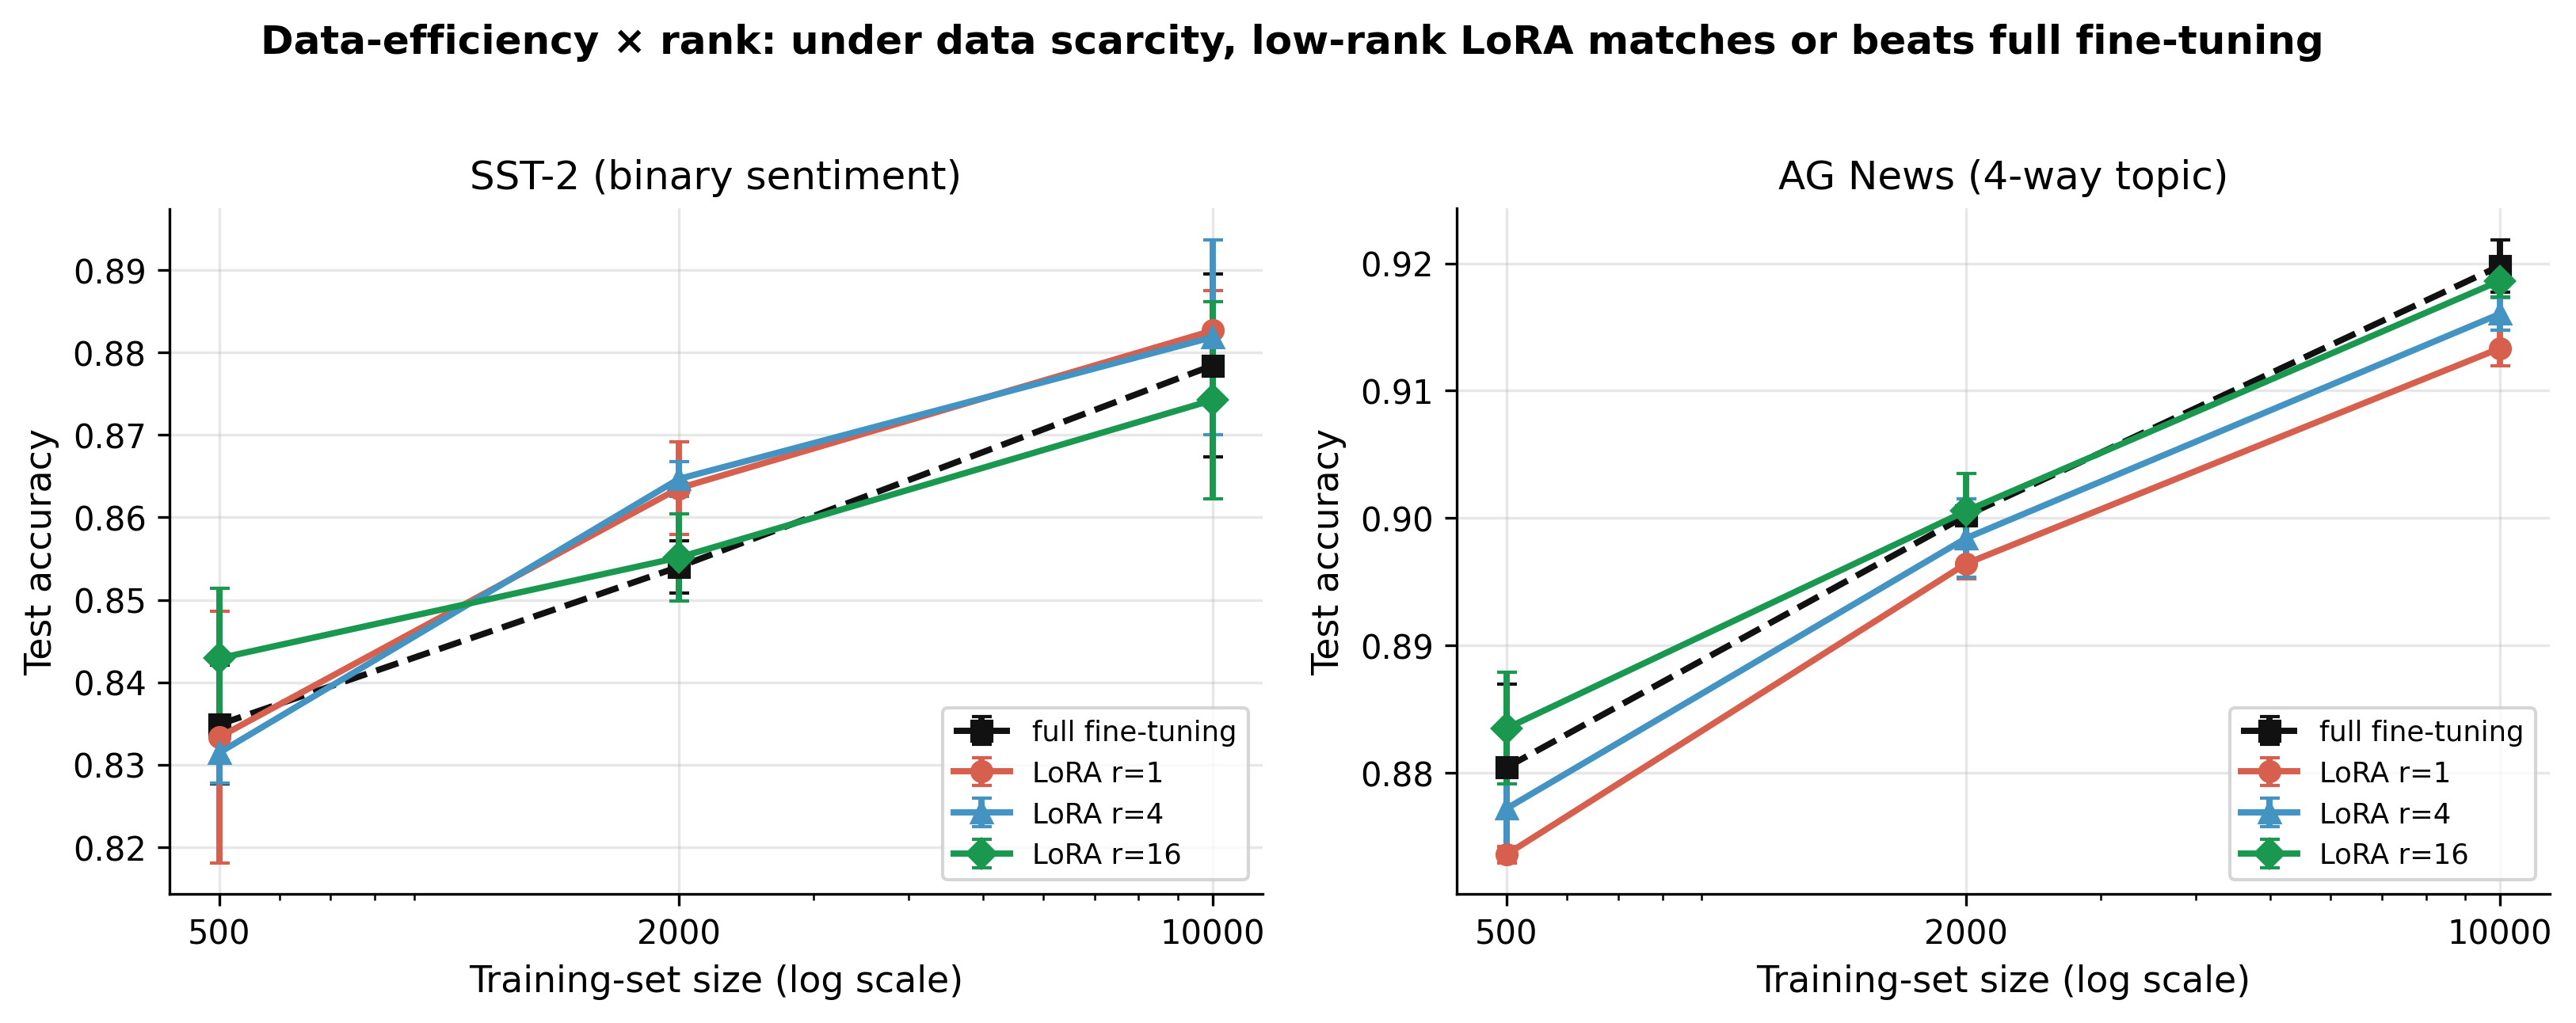
\includegraphics[width=0.95\textwidth]{figures/output/fig6_data_efficiency.png}
\caption{Data-efficiency study. Accuracy versus training-set size (log scale) for full fine-tuning and LoRA at $r \in \{1,4,16\}$. Under data scarcity, low-rank LoRA matches or beats full fine-tuning.}
\label{fig:dataeff}
\end{figure*}

\subsection{Discussion}
Three findings emerge. First, the only regime in which adaptation truly breaks down is rank 0: the probe is decisively worse than full fine-tuning, by 5.8 points on SST-2 and 2.9 points on AG News, while every rank $r \geq 1$ recovers most or all of the gap. The low-rank update therefore performs real, necessary work. Second, task difficulty sets the floor: the easy binary task saturates at $r{=}4$, while the harder four-way task requires $r{=}32$ for strict statistical equivalence. Third, the reported floor depends materially on the equivalence criterion. Because AG News has very small seed variance, sub-point accuracy gaps become statistically significant even though they are practically negligible, so the strict floor ($r{=}32$) and the practical floor ($r{\approx}4$) differ by nearly an order of magnitude. This distinction, invisible to studies that report only point estimates, is a methodological caution for the field: claims about the sufficiency of a given rank should state both the seed variability and the equivalence threshold.

\FloatBarrier
\section{Limitations and Future Work}
\label{sec:limitations}
Our study covers one backbone family (DistilBERT) and two classification tasks, and addresses encoder classifiers rather than generative decoders, where prior work~\cite{biderman2024lora} shows higher-rank demands on hard tasks. The minimum viable rank is defined relative to a chosen significance level and seed count; larger seed counts would tighten the confidence intervals and could shift the strict floor. Future work should extend the protocol to additional encoders such as DistilRoBERTa and BERT-base, to regression, natural-language-inference, and token-level tasks, and to decoder language models, and should study automatic per-layer rank allocation under the same significance-grounded lens.

\section{Conclusion}
\label{sec:conclusion}
We presented a statistically grounded study of how low the LoRA rank can go for small transformer encoders. The rank floor is astonishingly low and tracks task difficulty: a minimum viable rank of 4 on SST-2 and 32 on AG News under strict statistical equivalence, or approximately 4 under a practical tolerance, with even rank 1 (0.027\% of parameters) closing most of the gap to full fine-tuning. The only true breakdown occurs at rank 0, and the floor is robust to the scaling rule and to data scarcity, where low-rank LoRA matches or exceeds full fine-tuning. Practitioners can adapt DistilBERT-class models with on the order of 0.1\% trainable parameters at no statistically meaningful accuracy cost.

\section*{Acknowledgments}
The authors thank Vizuara AI Labs for providing mentorship and computational resources for this research.

\begin{thebibliography}{99}
\bibitem{hu2021lora} E. J. Hu, Y. Shen, P. Wallis, Z. Allen-Zhu, Y. Li, S. Wang, L. Wang, and W. Chen, ``LoRA: Low-rank adaptation of large language models,'' in \textit{Proc. ICLR}, 2022.
\bibitem{aghajanyan2020intrinsic} A. Aghajanyan, L. Zettlemoyer, and S. Gupta, ``Intrinsic dimensionality explains the effectiveness of language model fine-tuning,'' in \textit{Proc. ACL}, 2021.
\bibitem{li2018intrinsic} C. Li, H. Farkhoor, R. Liu, and J. Yosinski, ``Measuring the intrinsic dimension of objective landscapes,'' in \textit{Proc. ICLR}, 2018.
\bibitem{zhang2023adalora} Q. Zhang, M. Chen, A. Bukharin, P. He, Y. Cheng, W. Chen, and T. Zhao, ``AdaLoRA: Adaptive budget allocation for parameter-efficient fine-tuning,'' in \textit{Proc. ICLR}, 2023.
\bibitem{dettmers2023qlora} T. Dettmers, A. Pagnoni, A. Holtzman, and L. Zettlemoyer, ``QLoRA: Efficient finetuning of quantized LLMs,'' in \textit{Proc. NeurIPS}, 2023.
\bibitem{liu2024dora} S.-Y. Liu, C.-Y. Wang, H. Yin, P. Molchanov, Y.-C. F. Wang, K.-T. Cheng, and M.-H. Chen, ``DoRA: Weight-decomposed low-rank adaptation,'' in \textit{Proc. ICML}, 2024.
\bibitem{kopiczko2023vera} D. J. Kopiczko, T. Blankevoort, and Y. M. Asano, ``VeRA: Vector-based random matrix adaptation,'' in \textit{Proc. ICLR}, 2024.
\bibitem{kalajdzievski2023rslora} D. Kalajdzievski, ``A rank stabilization scaling factor for fine-tuning with LoRA,'' \textit{arXiv:2312.03732}, 2023.
\bibitem{biderman2024lora} D. Biderman, J. Portes, J. J. G. Ortiz, et al., ``LoRA learns less and forgets less,'' \textit{Trans. Machine Learning Research}, 2024.
\bibitem{rathore2025rank} D. Rathore, V. Kumar, C. Bansal, and A. Moitra, ``How much is too much? Exploring LoRA rank trade-offs for retaining knowledge and domain robustness,'' in \textit{Findings of IJCNLP-AACL}, 2025.
\bibitem{sanh2019distilbert} V. Sanh, L. Debut, J. Chaumond, and T. Wolf, ``DistilBERT, a distilled version of BERT: smaller, faster, cheaper and lighter,'' in \textit{NeurIPS EMC$^2$ Workshop}, 2019.
\bibitem{lialin2023scaling} V. Lialin, V. Deshpande, and A. Rumshisky, ``Scaling down to scale up: A guide to parameter-efficient fine-tuning,'' \textit{arXiv:2303.15647}, 2023.
\bibitem{xin2024survey} Y. Xin et al., ``Parameter-efficient fine-tuning in large models: A survey of methodologies,'' \textit{arXiv:2410.19878}, 2024.
\bibitem{houlsby2019adapter} N. Houlsby, A. Giurgiu, S. Jastrzebski, B. Morrone, Q. de Laroussilhe, A. Gesmundo, M. Attariyan, and S. Gelly, ``Parameter-efficient transfer learning for NLP,'' in \textit{Proc. ICML}, 2019.
\bibitem{wang2018glue} A. Wang, A. Singh, J. Michael, F. Hill, O. Levy, and S. R. Bowman, ``GLUE: A multi-task benchmark and analysis platform for natural language understanding,'' in \textit{Proc. ICLR}, 2019.
\bibitem{socher2013sst} R. Socher, A. Perelygin, J. Wu, J. Chuang, C. D. Manning, A. Y. Ng, and C. Potts, ``Recursive deep models for semantic compositionality over a sentiment treebank,'' in \textit{Proc. EMNLP}, 2013.
\bibitem{zhang2015agnews} X. Zhang, J. Zhao, and Y. LeCun, ``Character-level convolutional networks for text classification,'' in \textit{Proc. NeurIPS}, 2015.
\bibitem{devlin2019bert} J. Devlin, M.-W. Chang, K. Lee, and K. Toutanova, ``BERT: Pre-training of deep bidirectional transformers for language understanding,'' in \textit{Proc. NAACL}, 2019.
\bibitem{liu2019roberta} Y. Liu, M. Ott, N. Goyal, J. Du, M. Joshi, D. Chen, O. Levy, M. Lewis, L. Zettlemoyer, and V. Stoyanov, ``RoBERTa: A robustly optimized BERT pretraining approach,'' \textit{arXiv:1907.11692}, 2019.
\end{thebibliography}

\end{document}
